\documentclass[11pt]{article}
\usepackage{graphicx}
\usepackage{hyperref}
\usepackage{natbib}
\usepackage{indentfirst}
\setlength{\textwidth}{6.5in}
\setlength{\headheight}{0in}
\setlength{\textheight}{8.0in}
\setlength{\hoffset}{0in}
\setlength{\voffset}{0in}
\setlength{\oddsidemargin}{0in}
\setlength{\evensidemargin}{0in}
\title{ML Problem set 1}
  
\author{Krishna N. Dindial }


\begin{document}


\maketitle
\section{Github}
\url{https://github.com/kdindial/ML_Spring26.git}

\section{Problem 1}

To me, it seemed the best way to make model that is 
invariant to reflections is to make a model where the final output is to forced it to be even.
\begin{equation}
    f(x)=\frac{g(x)+g(-x)}{2}
\end{equation}

\par
My plan was to make some MLP model g(x), apply the symmetrizing function, then validate the loss using the symmetrized version of g, then update the weights and repeat.
I asked chatgpt how to do this, and it told me that in pytorch, you can build your neural network g, and then define a "forward pass function" that returns the symmetrized version of g.

\par
for the first toy model I tried to get it to learn the function:
\begin{equation}
    f(x)=-.4x^2+\sin{x}^2
\end{equation}

I generated some random x values between -2 and 5 as the training x values. I applied f(x) to the training x values without adding any noise to make the training y data.
\begin{center}
    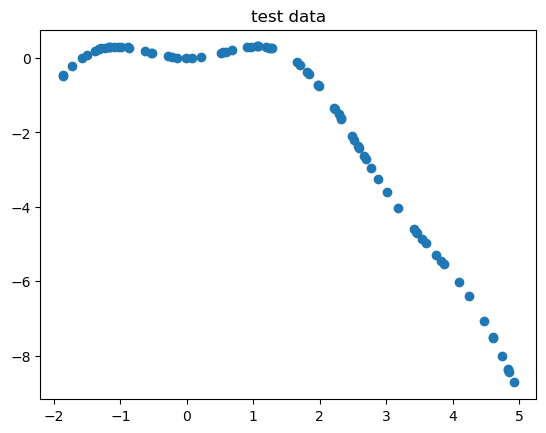
\includegraphics[width=0.6\linewidth]{figs/toytrain1.png}
\end{center}

I started with the non symmetrized model from sci kit learn. It was was a multi layer perceptron model with 2 layers with size 32.
I also trained a MLP model with 2 layers of size 32, but I used pytorch to symmetrize the model on the forward pass. I made the test data 100 points uniformly spread between
-4 and 4. Here is the performance
\begin{center}
    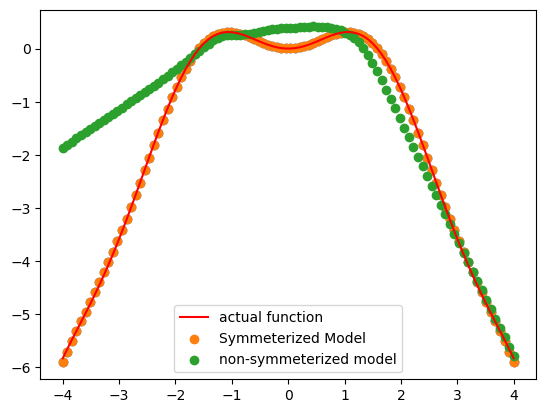
\includegraphics[width=0.6\linewidth]{figs/toymodel1.png}
\end{center}

The symmetrized model greatly outperformed the unsymmetrized one. The unsymmetrized loss was "74" while the symmetrized loss was "0.0043"
For a second toy model I tried a more "wiggly" function:

\begin{equation}
    h(x)=-.5x^2+2\sin{2x}^2
\end{equation}

I also added some noise ranging from 0 to 1 to the training y values:

\begin{center}
    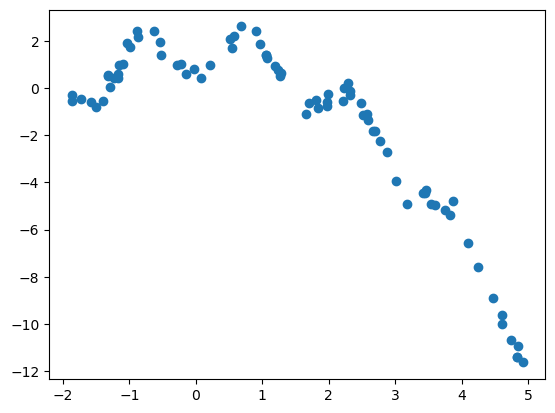
\includegraphics[width=0.6\linewidth]{figs/toytrain2.png}
\end{center}

I ran it through the same two nueral networks and here were the results:

\begin{center}
    
    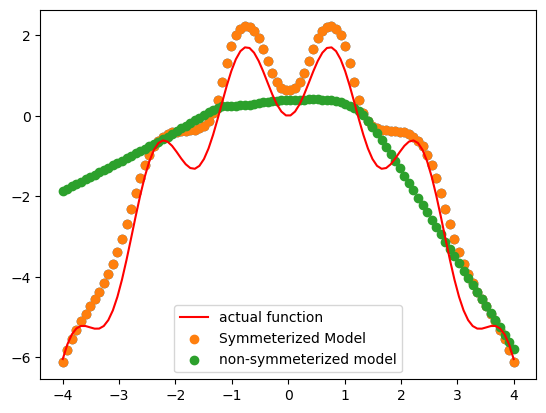
\includegraphics[width=0.6\linewidth]{figs/toymodel2.png}
\end{center}

Both models performed less well on this version, but the symmetrized model still outperformed the unsymmetrized model by
a factor of over 200. The unsymmetrized loss was around 88 and the symmetrized loss was around .4

\section{Problem 2}
\subsection{part 1}
For question 2 I will be using the turbulent radiative layer in 2D, as this is the only data set from the well that I could find that was under 50GB. 
Also it the tutorials from Clark and the web page for the well all used this data set
so it felt more comfortable because I am unfamiliar with this kind of physics and I also do not have much experience with simulations. 
There are 4 differential equations that describe the gas:
\par
conservation of mass:
\begin{equation}
    \frac{\partial \rho}{\partial t} + \nabla \dot (\rho v) =0
\end{equation}

conservatin of momentum:
\begin{equation}
    \frac{\partial \rho v}{partial t} +\nabla(\rho vv+ P)=0
\end{equation}

conservation of energy

\begin{equation}
    \frac{\partial E}{\partial t} +\nabla ((E+P)v)=-\frac{E}{t_cooled}
\end{equation}

Ideal gas law:
\begin{equation}
E=\frac{P}{\gamma-1}
\end{equation}

\par 
Boundary conditions: the simulation is periodic in the x direction and there is 0 gradient in the y direction (open boundary condition).


\par
The simulation describes a cold, dense gas on the bottom and a hot dilute gas on top (top and bottom refers to the y direction). The hot and
and cold gasses are moving relative to each other at "highly subsonic velocities". The gasses mix and more gas is cooled than is heated.

\par
There are 101 time steps and each image is 384 pixels (y direction) by 128 pixels (x direction). 
The data avilable is a density field (2D scalar field), a pressure field (2D scalar field) an
velocity field (2D vector field).

\par
Boundary conditions: The data is periodic at the x boundary $(f(x+L_x)=f(x))$ and there is zero gradient in the y boundary (open boundary conditions).

\par
Because of the periodic boundary condition it seems most natural to enforce translation equivariance in x. 
If you shift the whole simulation in the x direction and let it wrap around the boundary, then the final output should also have the same shift.

\subsection{part 2}

In the tutorial \hyperref{https://polymathic-ai.org/the_well/tutorials/dataset/}, they use an FNO.
I read this blog post \hyperref{https://zongyi-li.github.io/blog/2020/fourier-pde/} associated with this paper \hyperref{arXiv:2010.08895}.
The blog post mentions that the Fourier layer on its works only with periodic boundary conditions, "the Fiyruer network operator as a whole does not have these limitations".
\par
I will try to prove that the Fourier nueral Operator is translation equivariant. 
In \hyperref{arXiv:2010.08895} by Li et al, they start by defining the iterative updates where x is our data and v is some function of x. we want to predict how v will evolve as a function of x :

\begin{equation}
    v_{t+1}(x)=\sigma(Wv_t(x)+ (\kappa(a;\phi)v_t)(x))
\end{equation}

Where $\kappa$ is the kernel operator parameterized by phi, W is a linear transformation and sigma is the non linear activation
function

The Fourier Neural operator sets $\kappa$ to:
\begin{equation}
    (\kappa(\phi)v_t)(x)=F^{-1}(R_{\phi}(F(vt)(x)))(x)
\end{equation}
Where F is the Fiyruer transform and $R_{\phi}$ is the fourier transform of some periodic function. 
so to prove this is translation equivariant we would prove that the linear map W is translation equivariant, 
the fourier transform is translation equivariant.
\par since W is a linear map, we know:
\begin{equation}
    W(T_av(x))=W(v(x-a))=Wv(x-a)=t_a(Wv)(x)
\end{equation}

For the Fiyruer transform part, we know it is equivariant because we take the Fiyruer transform, multiply by some function in frequency space that does not depend on x, then take the inverse fourier transform. That must be translation equivariant.

\subsection{part 3}
This is probably the most important part of the problem set but I ran out of time! 
\end{document}

